As was described in section \ref{subsection:dl} the choice of the model architecture fell onto the UNet structure. Here will be provided a detailed decription of the architecture and the different layers used. An architecture used in this research was chosen based on paper [cite LaChance]. The input to this network is a $256 \times 256$-pixel DIC image that should be already preprocessed based on the corresponding to the desired organelle preprocessing pipeline. Specifications about different preprocessings are described separately in the next subsections dedicated to different organelles.

The encoder part of the UNet (Figure \ref{fig:unet}) step by step compresses spatial dimensions of the image (the spatial dimension size is detoned by a number on the left of each green block) into tensors or so-called feature maps with an increasing amount of filters (number of filters is denoted on the top of each green block). This allows to reduce the spatial information in the image and capture semantics. Decoder part on the contrary decompresses feature maps gradually increasing the amount of spatial information in tensors and reducing the number of filters. All convolutional layers use convolutions of size $3 \times 3$ with the corresponding number of filters. Downsampling in encoder reduces the spatial dimension twice during each step and implemented using max-pooling with a size of $2 \times 2$. Upsampling in decoder increases the spatial dimension also twice during each step and is implemented using transposed convolutions with a size of $2 \times 2$. After the first convolutional, that follows each max-pooling step, a batch normalization layer was used as it is well-known for speeding up the training process [cite Ioffe]. One should not forget though that using batch normalization might be sometimes dangerous due to the hidden information leaks it induces [cite Fetterman 2020]. Additionally dropouts were used for example for actin predictions as the model would encounter overfit quite easily there, however in the default architecture dropouts are not pressent. That is another thing that differs this architecture from the original one in [TODO Cite LaChance] paper. The last layer of the UNet here is a sigmoid activation function.
\begin{figure}[htb]
	\begin{center}
		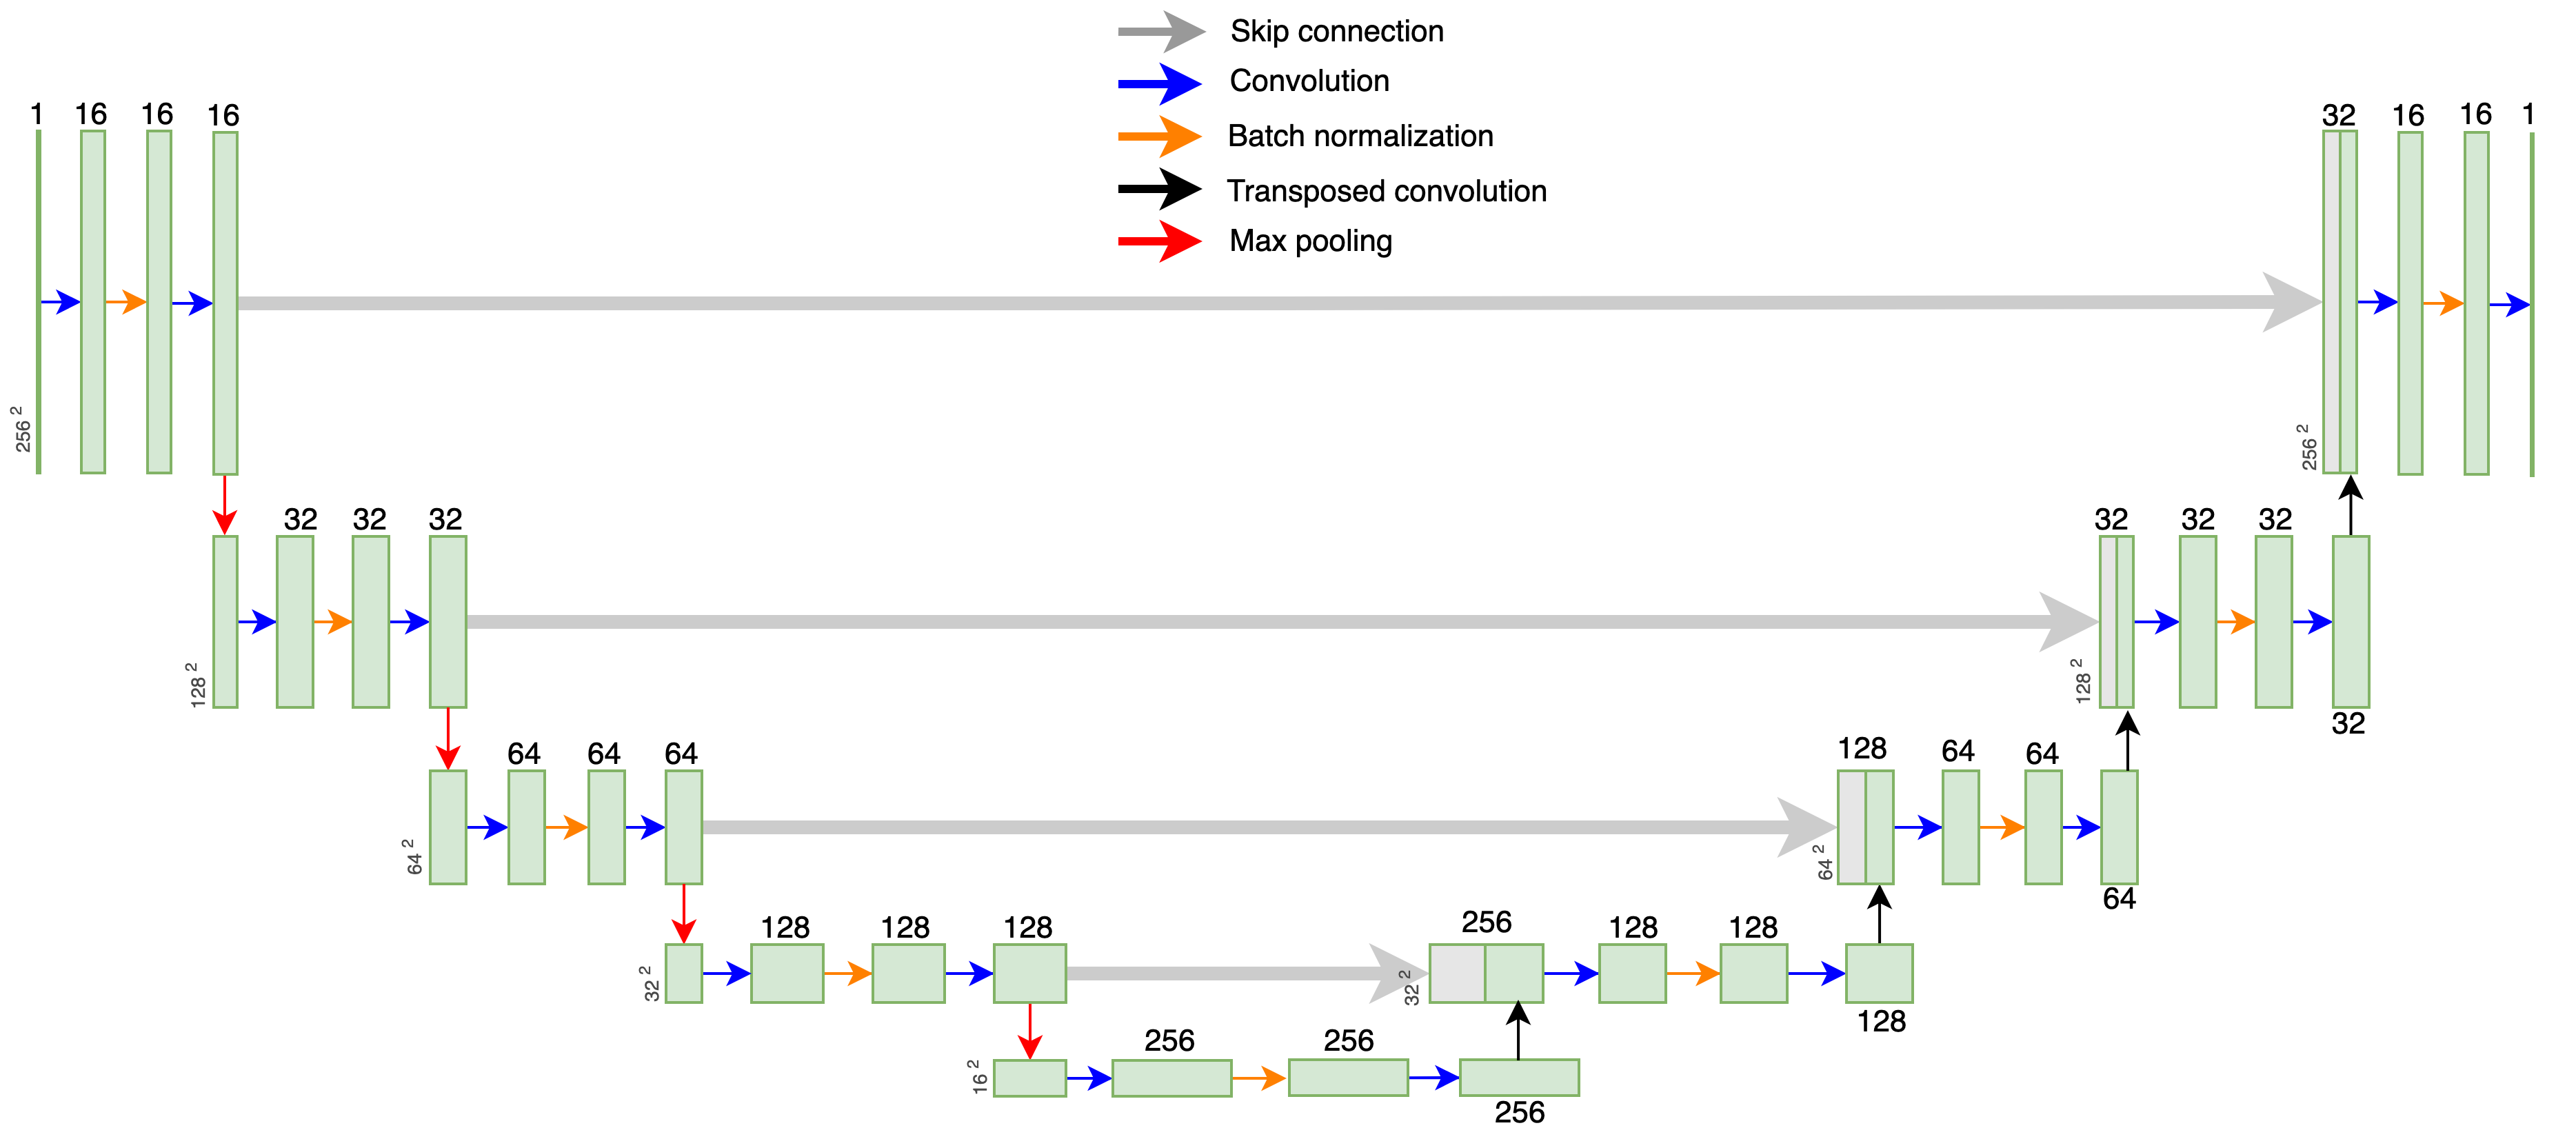
\includegraphics[width=\linewidth]{bilder/Unet.png}
		\caption{Unet}\label{fig:unet}
	\end{center}
\end{figure}

There is a space for potential improvements regarding the model architecture used in this research: for example, [Shiyui 2021] recommends to use special dense-block after each convolutional layer. They consist of another 3 convolutional layers with 24 filters, batch normalization layer and ReLU activations each. This could potentially facilitate efficient training of the model, still most probably the efficience comes mostly from Batch normalization layers that are already used in our architecture. Nethertheless the idea of using a bigger model such as one in [Shiyui 2021], or more specifically a model with more filters, indeed improves the predictions (shown in Section [TODO ref section]). That leaves the place available for further research and improvements regarding the size of the model and additional use of dense-blocks. 

An interesting question that automatically rises here is what do UNet embeddings (output tensors from the encoder) represent. There is a big difference between any representation learning network such as an autoencoder and a UNet --- a UNet model uses skip-connections that allow to propagate information between its encoder and a decoder. Meaning that embeddings do not contain purely semantic information, because essentially the network is not pushed towards compressing the information severely (as an autoencoder would do), but it should only extract relevant for segmentation features. One of the questions solved in this work was wether or not UNet embeddings are clustering based on the following classes: cell phenotypes, any kind of corruption within the data. For example, it would be bery usefull to be able to not only predict the data itselt, but also to say wether the prediction is reliable of not. The initial hypothesis here would be that if the predictions are not of a good enough quality this would be also reflected in the embeddings. 